\documentclass{article}
\usepackage{parskip}
\usepackage{graphicx}
\usepackage[margin=.6in]{geometry}
\begin{document}
\section*{Risk}
\label{sec:risk}
\subsubsection*{Introduction}
\label{ssub:introduction}


Social contracts involve envisioning how to help people thrive and then designing to help bring that about\\
It is often unclear how things will turn out\\
Design assessment should take account of uncertainty\\
Risk is one concept developed for this purpose\\
Principles of distribution include collectivism, equity, and individualism\\
\subsubsection*{Case study: Semi-automated cars}
\label{ssub:case_study_semi_automated_cars}


Donald Norman has argued against partial automation of driving, e.g., automatic lane-following and cruise controls\\
These lead to driver inattention and inability to cope with unusual situations\\
{Donald Norman}


Norman now argues that partial automation is acceptable\\
Risks of distraction exceed risks of inattention\\
Some inattention is a worthwhile trade-off\\
Alternatively, drivers might be required to use a “drive mode” on their smart phones\\
Which solution would be better?\\
\subsubsection*{Risks}
\label{ssub:risks}


Roughly speaking, risk = danger\\
Risks have several characteristics, including\\
Uncertainty\\
Comparability\\
These characteristics lead to risk trade-offs\\
E.g., crossing the street\\
\subsubsection*{A formal model of risk}
\label{ssub:a_formal_model_of_risk}


The “expected-value” model of risk:\\
Risk of event = (Probability of event)  (Severity of event)\\
E.g., average risk of a fall on stairs that requires hospitalization\\
Probability: 1/3,616,667\\
Severity: \$5567 (Canada, 2013)\\
Risk = (1/3,616,667) × (\$5567) = \$0.00154\\
Severity may be measured in \$ for market goods\\
Problematic where non-market goods are concerned\\
\subsubsection*{Safety trade-offs}
\label{ssub:safety_trade_offs}


Safety features can be used to decrease risk\\
However, safety features sometimes decrease one risk but increase another one\\
E.g., red-light cameras appear to decrease t-bone collisions but increase rear-end collisions\\
Red-light cameras result in a risk trade-off\\
Many argue that the trade-off is a good one\\
What other safety features involve risk trade-offs?\\
\subsubsection*{Collectivism}
\label{ssub:collectivism}

{Sven Ove Hansson}


When is a trade-off acceptable?\\
When it provides the best, overall outcome\\
The collectivist principle (Hansson):\\
Collectivism: An option is acceptable to the extent that the sum of all individual risks that it gives rise to is outweighed by the sum of all individual benefits that it gives rise to.\\
That is, the option serves the common good\\
Collectivism requires that some people pay a price for the good of others\\
\subsubsection*{Externalities}
\label{ssub:externalities}


The importance of the principle can be explored in cases where it is not observed\\
Consider the use of external A/C units in apartment block design, instead of central air\\
They are cheaper for designer and client but impose extra noise on occupants and neighbours\\
Noise pollution is a risk imposed on third parties, i.e., an externality\\
{What other design externalities can you think of?}


\subsubsection*{Equity}
\label{ssub:equity}


Endangering some people to help others may be problematic\\
The equity principle (Hansson):\\
Equity: An option is acceptable to the extent that it is part of a social system of risk-taking that is mutually advantageous and in which all participants enjoy equal latitude and consideration.\\
E.g., driving cars\\
All parties are allowed to impose risks on others\\
Others are allowed to impose similar risks on them\\
Certain risks are excluded, e.g., drunk driving\\
This arrangement is to everyone’s advantage\\
\subsubsection*{Equity as a social contract}
\label{ssub:equity_as_a_social_contract}


Equity involves a social contract\\
People enjoy a right to personal safety\\
People compromise this right so that everyone can realize a benefit, e.g., automotive mobility\\
This benefit promotes thriving\\
On the equity principle, the right to safety is fundamental\\
Rights play no role on the collectivist principle\\
A good design distributes risk equitably\\
\subsubsection*{Case study: Cyclist alert}
\label{ssub:case_study_cyclist_alert}


Equity implies that people in similar situations should face comparable risks\\
Thus, people who face unusual risks relative to others deserve particular measures\\
E.g., Jaguar’s in-car warning system regarding cyclists and pedestrians\\
What other examples of safety equipment increase equity?\\
\subsubsection*{Individualism}
\label{ssub:individualism}


Social trade-offs are not always appropriate\\
Consider the individualist principle (Hansson):\\
Individualism: An option is acceptable to the extent that the risk to which each individual is exposed is outweighed by benefits for that same individual\\
This principle applies to medical devices designed for therapy\\
{Population measures, e.g., vaccines, apply the equity principle}


\subsubsection*{Case study: Smart pacemakers}
Pacemakers are therapeutic devices designed to prevent heart attacks\\
Modern pacemakers are often Internet-accessible\\
Connectivity introduces security risks\\
Yet, the risks are outweighed by the benefits for individuals\\
What other risks do medical devices expose patients to? Why are they acceptable, or not?\\

\section*{Fairness}
\label{sec:fairness}
\subsubsection*{Introduction}
\label{ssub:introduction}
Conflicts of interest may exist between social groups\\
Interest: something that may be gained or lost\\
Conflict: A gain for one group is a loss for the other\\
Fairness involves appropriate balance between conflicting interests\\
Designs can affect conflicting interests and give rise to fairness issues\\
Design assessment includes characterizing and addressing such fairness issues\\
\subsection*{Case study: LightAlert}
\label{sub:case_study_lightalert}
LightAlert is a “ghetto-avoider”\\
LightAlert alerts users when they approach the location of a previous assault or sexual assault\\
Its developers note that 20−25\% of US college women report being victims of sexual assault or attempted sexual assault\\
What kinds of mistakes would LightAlert make? What are some consequences of these errors for the people involved?\\
\subsection*{Fairness}
\label{sub:fairness}
Fairness means balancing legitimate and competing interests of different social groups\\
LightAlert involves two groups with such interests:\\
Users who want to remain safe\\
Residents who want to avoid stigmatization\\
Fairness issues relate to assumptions in design\\
What assumption does LightAlert make to perform accurately?\\
\subsection*{Predictions and accuracy}
\label{sub:predictions_and_accuracy}
Designs rely on assumptions about the future: predictions\\
Accuracy of a prediction is the frequency with which it is correct\\
Represented by a correlation [0..1]\\
Data can be represented on a scatter plot\\
X-axis (predictions)\\
Y-axis (events)\\
Accuracy is measured by the smallest ellipse around data points\\
E.g., 0.2, 0.5, 0.8\\
\subsection*{The Taylor-Russell diagram}
\label{sub:the_taylor_russell_diagram}
The Taylor-Russell diagram provides a general model of error in design\\
Design threshold (horizontal line): divides events that require different actions or responses\\
Prediction cutoff (vertical line): divides predictions that indicate the need for different actions or responses\\
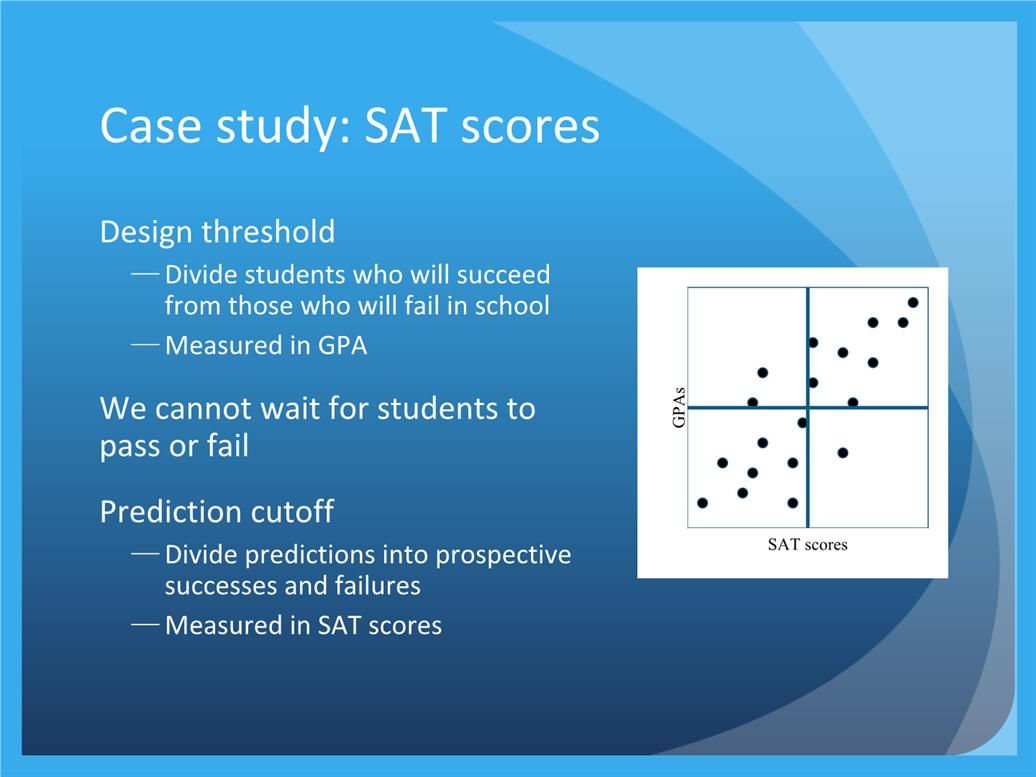
\includegraphics[scale=0.5]{russelldiagram.jpg}
\subsection*{Case study: SAT scores}
\label{sub:case_study_sat_scores}
Design threshold\\
Divide students who will succeed from those who will fail in school\\
Measured in GPA\\
We cannot wait for students to pass or fail\\
Prediction cutoff\\
Divide predictions into prospective successes and failures\\
Measured in SAT scores\\
\subsection*{Kinds of results}
\label{sub:kinds_of_results}
The threshold and cutoff divide the plot into four quadrants\\
False positive (LR): design decision is made but proves unnecessary\\
False negative (UL): design decision is not made but proves necessary\\
Consider the SAT test again:\\
False positive: Students are admitted but fail\\
False negative: Students are rejected but would have succeeded\\
\subsection*{Trade-off between errors}
\label{sub:trade_off_between_errors}
Error types are inextricably linked\\
Moving the cutoff to reduce one kind increases the other kind\\
SAT tests:\\
Move the cutoff right to reduce false positives in University admissions\\
More students who would have succeeded will be denied admission (false negatives)\\
\subsection*{Error and values}
\label{sub:error_and_values}
Which error would it be better to make?\\
It depends on the value you place on each kind\\
Different social groups will value each error type differently (Hammond 1996)\\
E.g., taxpayer groups will argue that too many students who go to University do not graduate\\
Parents will argue that too few graduates are available for a competitive economy\\
The prediction cutoff oscillates as policy makers try to satisfy each constituency\\
\subsection*{Error and fairness}
\label{sub:error_and_fairness}
Errors pit the interests of constituencies against each other\\
This outcome creates an issue of fairness:\\
Who ought to benefit or suffer from mistakes arising from design assumptions?\\
How should competing interests be balanced?\\
\subsection*{Fairness and LightAlert}
\label{sub:fairness_and_lightalert}
A fairness assessment for LightAlert can begin with a T-R diagram\\
False positive (LR): Safe areas are unnecessarily avoided and acquire an undeserved reputation.\\
False negative (UL): Women relying on LightAlert unwittingly enter a dangerous area.\\
View as PageDownloadToggle Fullscreen\\
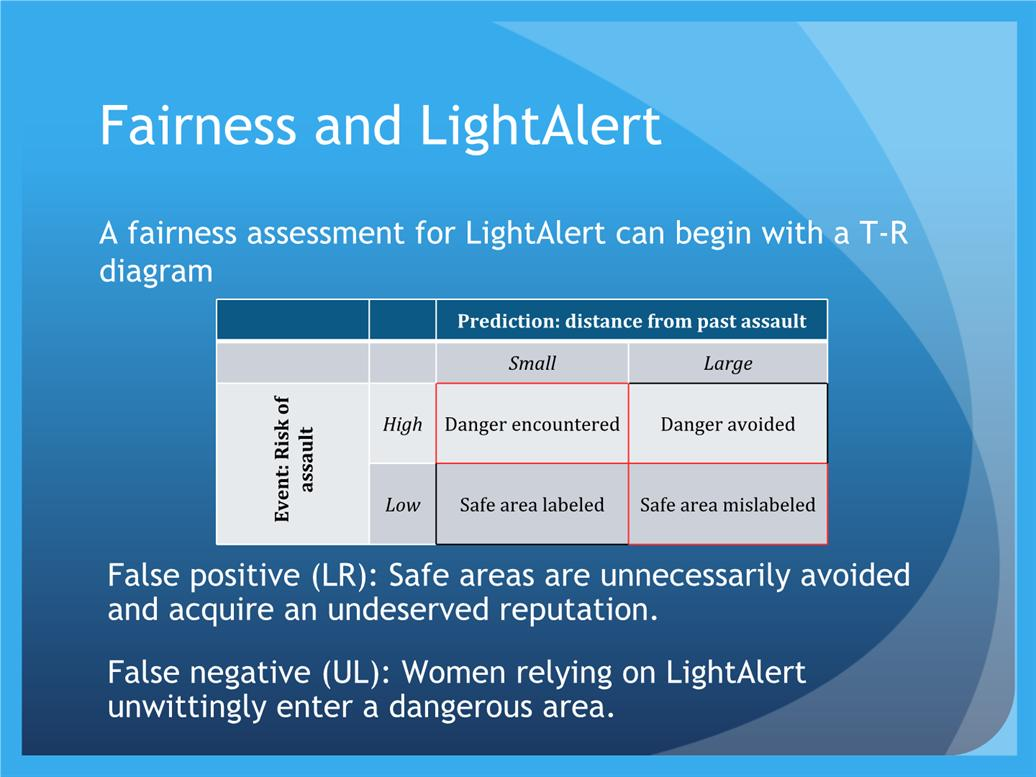
\includegraphics[scale=0.5]{errorandfairness.jpg}


\section*{Progress}
\label{sec:progress}
\subsubsection*{Introduction}
\label{ssub:introduction}
Progress means that things improve over time\\
Besides technical progress, there may be moral progress (Simon):\\
“Moral progress has always been associated with the capacity to respond to universal values—to grant equal weight to the needs and claims of all mankind, present and future.”\\
To simplify, consider: Would it be fair to accept or restrict a new design?\\
\subsubsection*{Case study: Brain stimulation}
\label{ssub:case_study_brain_stimulation}
TDCS = Transcranial Direct Current Stimulation\\
Involves inducing brain activity through electrodes on the scalp\\
Some research suggests TDCS can be used to treat conditions such as depression, autism, Parkinson’s disease\\
DIY hackers have been using homebrew kits to treat themselves\\
E.g., Mr. Zobrist has treated his blindness\\
Such hacking carries potential risks\\
E.g., interactions, persistence, individual variation, side-effects\\
\subsubsection*{Thync}
\label{ssub:thync}
Startups are beginning to manufacture brain stimulators\\
Thync has a “calm” mode and an “energy” mode\\
On the plus side:\\
There have been positive user responses\\
A small study supports “calm” mode, a little\\
On the minus side:\\
Results may be idiosyncratic and unreliable\\
It is unclear what a safe stimulator would be\\
How should Thync be regulated? Restrictively, loosely, or in-between?\\
\subsubsection*{The concept of progress}
\label{ssub:the_concept_of_progress}
Progress = making things better than before\\
Better = more good\\
Since good is ambiguous, so is progress\\
Good design:\\
Rational: Good designs are ones that achieve their ends in excellent ways, whatever those are.\\
Moral: Good designs are ones that help to achieve excellent ends.\\
Progress in design:\\
Rational: Progress is made when designs become more excellent in the achievement of their ends, whatever those are.\\
Moral: Progress is made when designs help to achieve more excellent ends.\\
\subsubsection*{A dilemma of progress}
\label{ssub:a_dilemma_of_progress}
Adapt a Fairness Impact Assessment\\
Constituencies affected:\\
Critics worry about false positives\\
Advocates worry about false negatives\\
What social issue is involved?\\
\subsubsection*{Two strategies for regulation}
\label{ssub:two_strategies_for_regulation}
This example illustrates a general dilemma\\
Permissive: accept an innovation that is not proven unsafe\\
Precautionary: avoid an innovation until proven safe\\
The strategies are mutually exclusive\\
\subsubsection*{Climate change}
\label{ssub:climate_change}
The industrial revolution has been driven by energy obtained from fossil fuels\\
This practice has had the unintended consequence of climate change\\
The IPCC Fifth Assessment notes that, “Continued emission of greenhouse gases will cause further warming and long-lasting changes in all components of the climate system…”\\
It recommends drastic cuts to emissions\\
\subsubsection*{Geoengineering}
\label{ssub:geoengineering}
Geoengineering would re-design the climate to respond less to greenhouse gas inputs\\
Carbon capture: scrubbers to remove CO2 and store it\\
Solar radiation management: reflect some sunlight away from Earth\\
Critics worry about political problems and further unintended consequences\\

\section*{Sustainability}
\label{sec:sustainability}
\subsubsection*{Introduction}
\label{ssub:introduction}
Sustainability is a part of good design
\begin{itemize}
	\item It concerns the problem of regulating consumption in the face of limited resources\\
\end{itemize}
Sustainability presents a problem of moral progress
\begin{itemize}
	\item Maintain prosperity but prevent crises
\end{itemize}
Two strategies:
\begin{itemize}
	\item Growth, facilitated by efficiency
	\item Degrowth, facilitated by conservation
\end{itemize}
\subsubsection*{Case study: Shower heads}
\label{ssub:case_study_shower_heads}
Showering accounts for 17\% of US household water use (4.5 trillion liters/year, EPA)\\
Shower flow capped at 2.5 gallons/min. (U.S. Energy Policy Act of 1992)\\
Existing shower heads were fitted with flow restrictors\\
What factors might undermine this plan?\\
New low-flow shower heads may be fitted with aerators\\
\subsubsection*{Case study: Power drills}
\label{ssub:case_study_power_drills}
About half of American households have power drills\\
The average drill operates between 6 and 13 minutes over its lifetime\\
The Do-It-Yourself movement launched after WWII\\
Tool manufacturers designed lighter, less robust versions of professional tools for consumer market\\
Advertising promoted the image that any real man should also be a handyman\\
\subsubsection*{Case study: Neighborgoods.net}
\label{ssub:case_study_neighborgoods_net}
Neighborgoods allows people to borrow from and lend to their neighbors\\
Neighborgoods illusrates collaborative consumption (Botsman \& Rogers 2010)\\
De-emphasis on ownership and material culture\\
What are some other examples of collaborative consumption? What are some trade-offs?\\
\subsubsection*{Sustainability and progress}
\label{ssub:sustainability_and_progress}
Two strategies for progress:
\begin{itemize}
	\item Growth: encourage economic activity, e.g., through consumerism in design;\\
	\item Degrowth: encourage resource conservation and reduction of excess capacity, e.g., through CC\\
\end{itemize}
\subsubsection*{Industrialism}
\label{ssub:industrialism}
Industrialism emphasizes consumption
\begin{itemize}
	\item Conversion of resources into work and outputs
\end{itemize}
Heinberg’s (2007) axioms of sustainability include:
\begin{itemize}
	\item Consumption of renewables must occur at less than the rate of replenishment
	\item Consumption of nonrenewables must decline faster than the rate of depletion
\end{itemize}
Increasing efficiency extends consumption in the future\\
\subsubsection*{Jevons’ Paradox}
\label{ssub:jevons_paradox}
William Jevons’ “The coal question” (1865) argued that efficient engines would increase consumption\\
E.g., rail transportation\\
Predicted that Britain would run out of coal by the mid 20th century\\
William Jevons (1835–1882)\\
Two manifestations:
\begin{itemize}
	\item Rebound effect: some gains are lost to new consumption
	\item Backfire effect: gains are overwhelmed by new consumption
\end{itemize}
\subsubsection*{Explanations}
\label{ssub:explanations}
Three reasons for Jevons’ Paradox:
\begin{itemize}
	\item Direct: gains in efficiency lower unit cost of a resource, stimulating consumption of it
	\item Indirect: Savings through efficiency in one resource stimulate consumption of another one
	\item Dynamic: Savings stimulate new modes of consumption
\end{itemize}
What indirect and dynamic effects could result from increased automotive efficiency?\\
\subsubsection*{Case study: Lighting}
\label{ssub:case_study_lighting}
People have responded more efficient lighting by consuming more power with it\\
Introduction of LED bulbs could increase average consumption from 46 Mlmh to 200 Mlmh by 2030 (Tsao 2010)\\
What indirect and dynamic effects could result from increased efficiency in lighting?\\
\subsubsection*{Biosynergism}
\label{ssub:biosynergism}
Promoting consumption that is more efficient in individual designs may not result in overall gains of sustainability\\
Biosynergism represents a systemic approach
\begin{itemize}
	\item Organicism: maintaining internal integrity
	\item Environmentalism: maintaining external integrity
\end{itemize}
Described by Scottish biologist Patrick Geddes (1854–1932)\\
\subsubsection*{Organicism}
\label{ssub:organicism}
Populations of organisms tend to fit into a “web of life”\\
A network of mutual interdependencies\\
Such networks exhibit synergy (Geddes)
\begin{itemize}
	\item The system supports each component
	\item The components each enhance sustainability of the system
\end{itemize}
Geddes argued that artificial systems should be designed to possess synergy\\
\subsubsection*{Case study: VanDusen Botanical Garden}
\label{ssub:case_study_vandusen_botanical_garden}
The new Visitor Centre exhibits synergistic design features, e.g.,\\
Waste from its toilets and food waste composted from its restaurants are combined and used as fertilizer for the plants in its gardens.\\
Wastewater is separated out and purified and used for irrigation in the gardens.\\
\subsubsection*{Environmentalism}
\label{ssub:environmentalism}
Synergism applies also to relationships between systems\\
Environmentalism: how well a system is integrated with others in its environment\\
Consider AquaFresco (MIT Water Innovation prize, 2015)\\
Reuses unused water and detergent from washing machines\\
“Current laundry technology is not sustainable. A regular washer discards the water right into the drain after one usage, but less than 1 percent is the actual waste component.”\\
\subsubsection*{Linear vs. circular}
\label{ssub:linear_vs_circular}
Architect John Tillman Lyle (1994) contrasts typical industrialist design with biosynergistic design\\
Industrialism\\
Biosynergism\\
What other biosynergistic (“circular”) designs can you think of?\\








\end{document}
